\documentclass{article}
% declares the document TYPE -- "article" is a simple class with no
% chapters, good default for short reports/papers (compare: "report",
% "book", "beamer" for slides)

\usepackage{booktabs}   % nicer table rules -- matches xtable's booktabs output
\usepackage{graphicx}

\title{Data Analytics -- Course Report}   % just STORES the title -- doesn't display it yet
\author{Vojtěch}                          % same -- stored for \maketitle to use later
\date{\today}                             % \today auto-inserts the current compile date

\begin{document}
	% everything ABOVE this line is the "preamble" (settings/packages, no
	% output); everything BELOW it is what actually gets typeset on the page
	
	\maketitle
	% NOW renders the title/author/date block using the three values
	% declared above -- this is the command that actually produces output
	
	\clearpage
	% forces a page break -- also flushes any pending floats (tables,
	% figures) before starting the new page. (compare: \newpage, a plain
	% page break that does NOT flush floats first)
	
	\tableofcontents
	% auto-generates a table of contents from your \section{}/
	% \subsection{} commands. GOTCHA: it needs to compile TWICE -- the
	% first run writes section names to a hidden .toc file, the second
	% run reads that file to actually build the list. if the TOC looks
	% empty or out of date after adding/renaming a section, just
	% recompile again
	
	\clearpage
	% another page break -- keeps the TOC on its own page, separate from
	% section 1
	
	\section{Statistics}
	% starts a new, automatically NUMBERED section with this heading
	
	Choosing the right statistical method depends on whether the data
	supports the normality assumption.
	% plain body text -- LaTeX treats a blank line as a paragraph break,
	% not a single newline (a lone line break is ignored)
	
	
	% latex table generated in R 4.4.2 by xtable 1.8-4 package
% Fri Sep 11 15:41:49 2026
\begin{table}[ht]
\centering
\begingroup\footnotesize
\begin{tabular}{lll}
  \toprule
question & parametric & nonparametric \\ 
  \midrule
comparing two groups & t-test & Mann-Whitney U \\ 
  comparing 3+ groups & ANOVA & Kruskal-Wallis \\ 
  relationship of two continuous variables & Pearson correlation / regression & Spearman correlation \\ 
  association of two categorical variables & Chi-square & Fisher's exact \\ 
   \bottomrule
\end{tabular}
\endgroup
\end{table}

	% pulls in another .tex file and inserts its content HERE, as if it
	% had been typed directly at this point in the document. no caption
	% or label is set here -- since there's no \begin{table} wrapper in
		% THIS file, whatever caption/label xtable produced (or didn't) on
		% the R side is what you get
		
		
		

	\subsection{Two-groups Comparison (t-test)}
	When we run a $t$-test, the sample data is condensed into a single number, the $t$-statistic, which measures how many standard errors the observed result sits away from what $H_0$ predicts. To turn that number into a $p$-value, R places it on a $t$-distribution -- a bell-shaped curve whose exact shape is governed by the degrees of freedom, $df = n - 1$. For small $df$ this curve has heavier tails than the normal distribution, reflecting the extra uncertainty that comes from estimating variance off a small sample; as $df$ grows, the $t$-distribution converges to the standard normal. The $p$-value is then simply the area under this curve beyond the observed $|t|$ (both tails, for a two-sided test), as shown in Figure~\ref{fig:tdist-pvalue}: a larger $|t|$ falls further into the tail, leaving less area beyond it, and hence a smaller $p$-value. Historically, this area was found by comparing $t$ against a critical value read off a printed table for the chosen significance level $\alpha$ and $df$ -- for a two-sided test at $\alpha = 0.05$, for instance, $t$ needs to fall at or beyond the $97.5^{th}$ percentile of the distribution (in absolute value), since the $5\%$ is split evenly across the two tails. Software now performs this same area calculation directly, which is why R reports a $p$-value rather than requiring a table lookup.
	
	\begin{figure}[h]
		\centering
		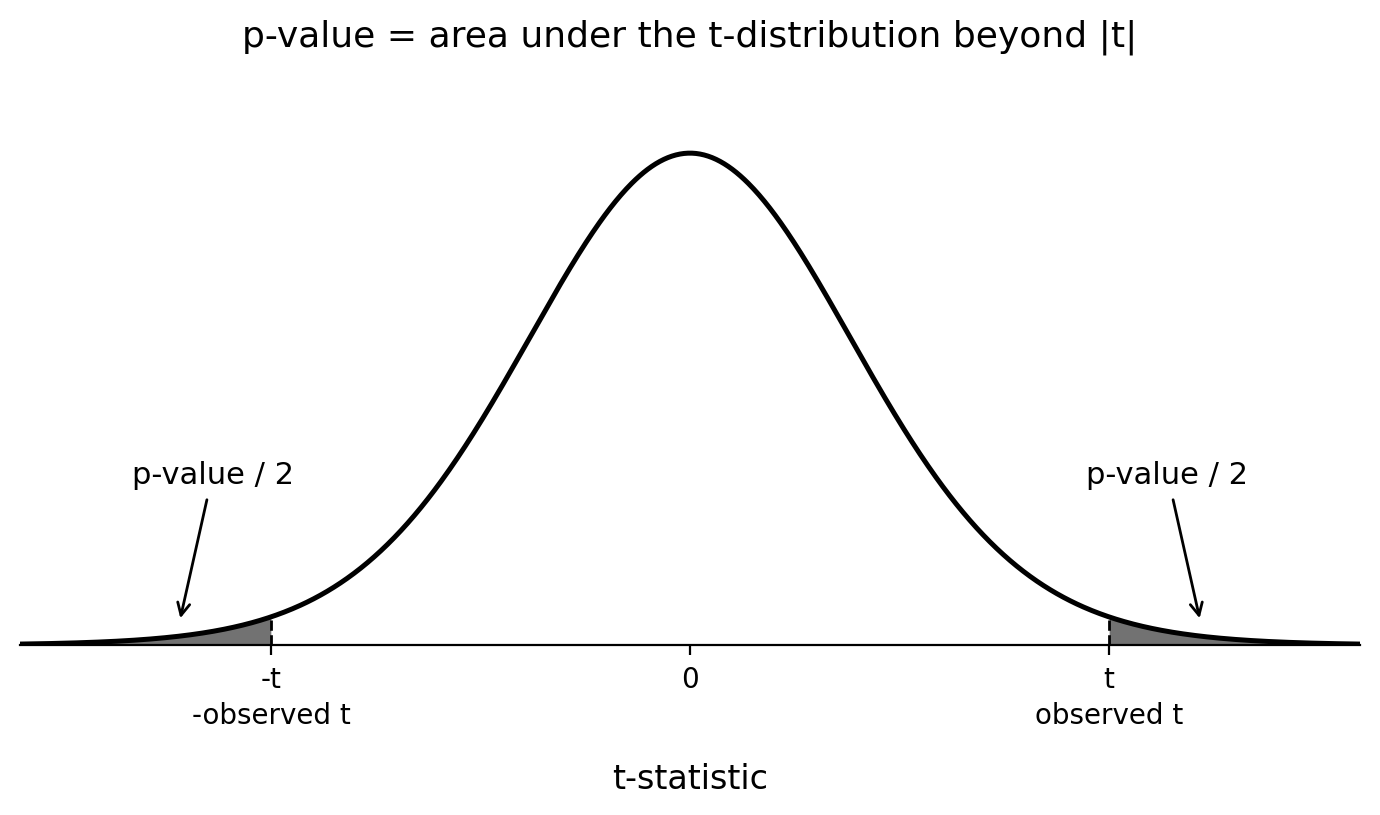
\includegraphics[width=0.7\textwidth]{manual-figures/t_distribution_pvalue}
		\caption{The $p$-value as the area under the $t$-distribution beyond the observed test statistic. The shaded regions in both tails together sum to the $p$-value; a larger $|t|$ pushes further into the tail, leaving less area beyond it, i.e., a smaller $p$-value.}
		\label{fig:tdist-pvalue}
	\end{figure}

		
	\end{document}
	% marks the end of the document -- anything typed after this line is
	% ignored by LaTeX entirely